%%%%%%%%%%%%%%%%%%%%%%%%%%%%%%%%%%%%%%%%%%%%%%%%%%%%%%%%%%%%%%%
% Set up document
%%%%%%%%%%%%%%%%%%%%%%%%%%%%%%%%%%%%%%%%%%%%%%%%%%%%%%%%%%%%%%%

\documentclass[xcolor={usenames,dvipsnames}]{beamer}
\usetheme{Madrid}
\setbeamersize{text margin left=5mm,text margin right=5mm}

% Dark background with non-white words: 
% \usecolortheme{owl}
% \setbeamercolor{normal text}{fg=yellow}
% \setbeamercolor{frametitle}{fg=yellow}
% \usebeamercolor[fg]{normal text}

% Used to create a section slide between section
\AtBeginSection[]{
  \begin{frame}[noframenumbering, plain]
  \vfill
  \centering
  \begin{beamercolorbox}[sep=8pt,center,shadow=true,rounded=true]{title}
    \usebeamerfont{title}\insertsectionhead\par%
  \end{beamercolorbox}
  \vfill
  \end{frame}
}

% Used to create a subsection slide between subsections
% \AtBeginSubsubsection{\frame{\subsubsectionpage}}
\AtBeginSubsection[]{
  \begin{frame}[noframenumbering, plain]
  \vfill
  \centering
  \begin{beamercolorbox}[sep=8pt,center,shadow=true,rounded=true]{title}
    \usebeamerfont{title}\insertsectionhead:\par\phantom{space please}\par\insertsubsectionhead\par%
  \end{beamercolorbox}
  \vfill
  \end{frame}
}


% Remove default navigation symbols and add just  page number
\setbeamertemplate{navigation symbols}{} % Clear default navigation
% \addtobeamertemplate{navigation symbols}{}{%
%     \usebeamerfont{footline}%
%     \usebeamercolor[fg]{footline}%
%     \hspace{1em}%
%     \insertframenumber/\inserttotalframenumber
% }

% Remove from footer the names, institution, date...
% and just leave page number:
\setbeamertemplate{footline}[frame number]


% For manual font size:
\usepackage{anyfontsize}

% For smaller URLs:
\newcommand{\smallurl}[1]{\textcolor{blue}{\fontsize{5pt}{5.8pt}\selectfont \url{#1}}}
%%%%%%%%%%%%%%%%%%%%%%%%%%%%%%%%%%%%%%%%%%%%%%%%%%%%%%%%%%%%%%%




% Title page
\title{Open science in the stroke projects}
\author{Anna Laws, Kerry Pearn, Michael Allen}
%\institute{Overleaf}
\date{November 2022}
\begin{document}
%\frame{\titlepage}

%%%%%%%%%%%%%%%%%%%%%%%%%%%%%%%%%%%%%%%%%%%%%%%%%%%%%%%%%%%%%%%


\begin{frame}
\titlepage
\end{frame}

%%%%%%%%%%%%%%%%%%%%%%%%%%%%%%%%%%%%%%%%%%%%%%%%%%%%%%%%%%%%%%%


\begin{frame}
\frametitle{Outline}
\tableofcontents
\end{frame}

%%%%%%%%%%%%%%%%%%%%%%%%%%%%%%%%%%%%%%%%%%%%%%%%%%%%%%%%%%%%%%%

\section{Stroke Projects}

\begin{frame}{The problem....}

\begin{center}
    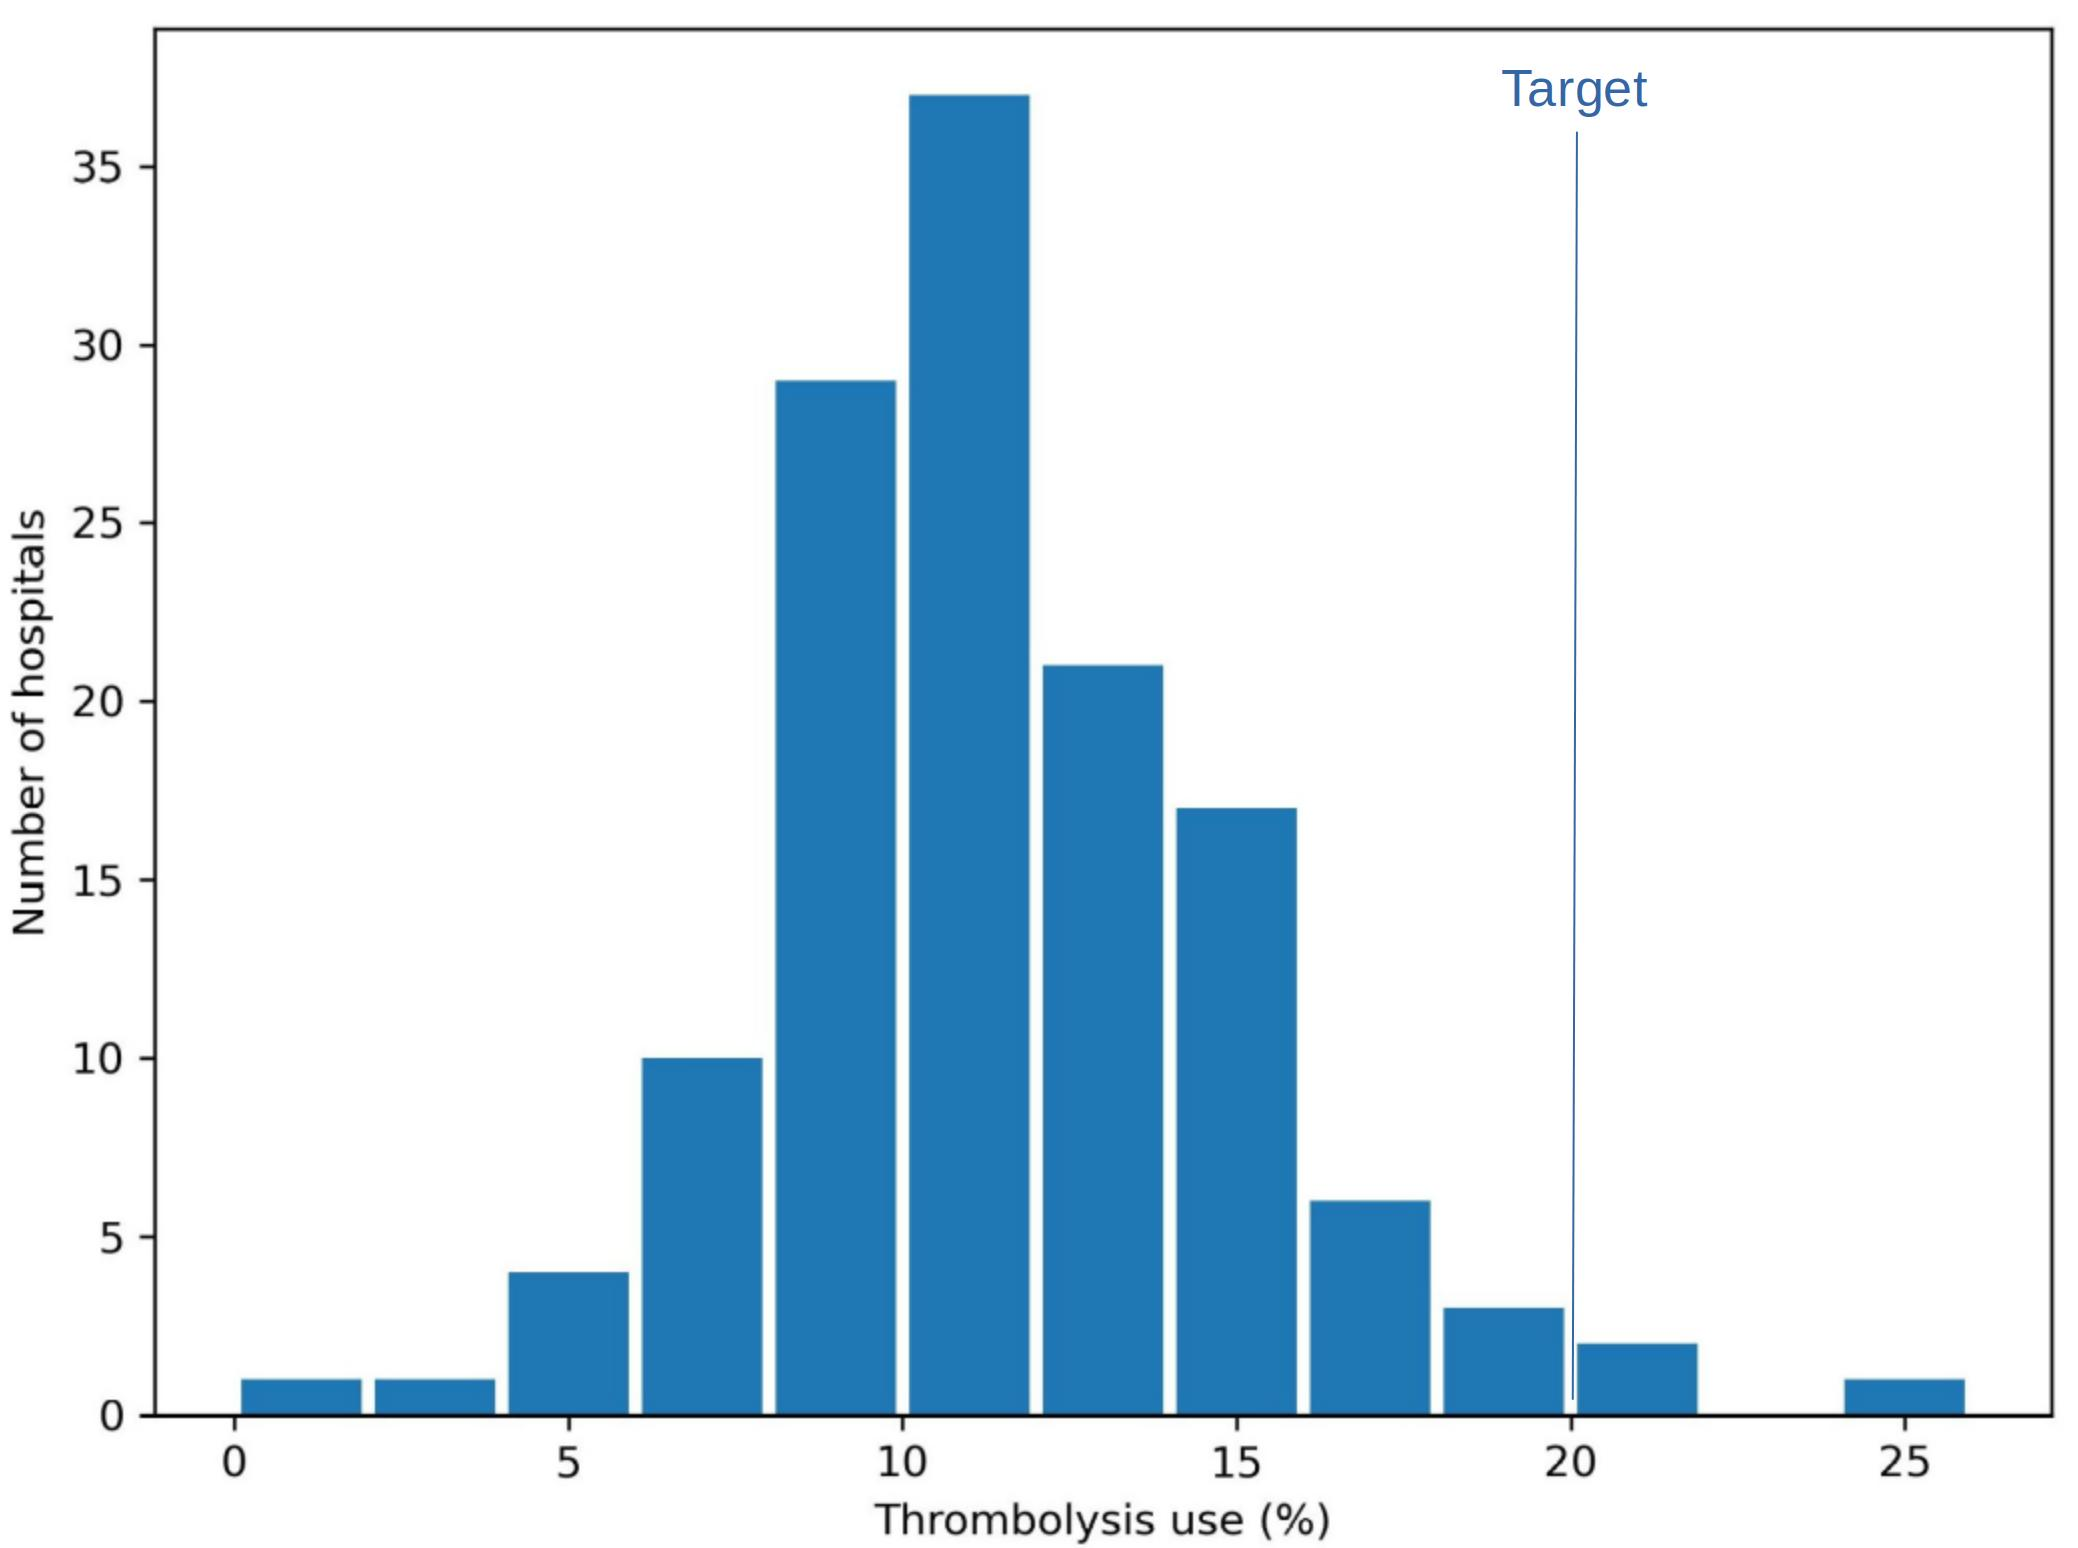
\includegraphics[width=0.65\textwidth]{./images/thrombolysis_by_hospital}
\end{center}
    
The central problem we are investigating is that there is a NHS target to give clot-busting drugs (\emph{thrombolysis}) to 20\% of patients, but actually only 11\% patients are receiving them (and this varies from 5\% to 25\% between hospitals).

\end{frame}



%%%%%%%%%%%%%%%%%%%%%%%%%%%%%%%%%%%%%%%%%%%%%%%%%%%%%%%%%%%%%%%



\begin{frame}{Stroke projects}
\begin{itemize}
    \setlength\itemsep{2.5mm}
    \item SAMueL: Stroke Audit Machine Learning 
    \begin{itemize}
        \item Emergency stroke clinical pathway simulation
        \item Machine learning to learn and compare clinical decision-making between hospitals
        \item Detailed (disability-level) clinical outcome model
        \item Health economics model
    \end{itemize}
    \item OPTIMIST: OPTimising IMplementation of Ischaemic Stroke Thrombectomy
        \begin{itemize}
            \item Modelling and optimising the pre-hospital emergency stroke pathway.
        \end{itemize}
    \item Mobile Stroke Units (hopefully!)
    \item Geographic modelling (update)
    \item Whole stroke system modelling?
\end{itemize}
\end{frame}

%%%%%%%%%%%%%%%%%%%%%%%%%%%%%%%%%%%%%%%%%%%%%%%%%%%%%%%%%%%%%%%

\section{SAMueL}

\begin{frame}
\frametitle{Breaking down the emergency stroke pathway into key steps}
\begin{center}
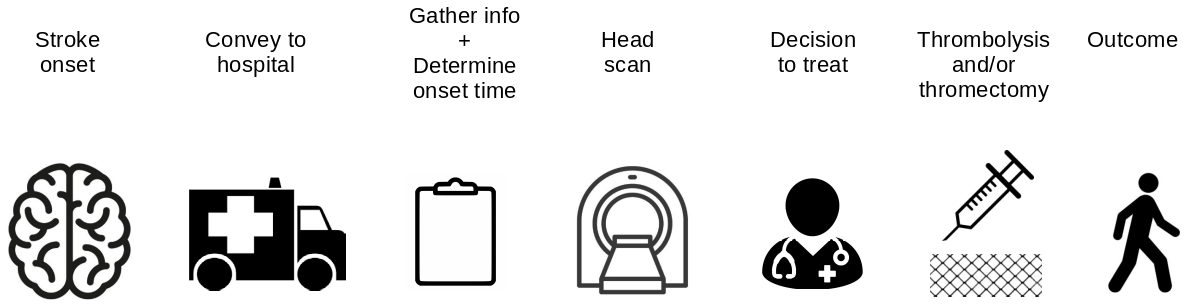
\includegraphics[width=0.90\textwidth]{./images/pathway_2}
\end{center}
We can model key changes to pathway:
\begin{small}
\begin{itemize}
    \item What if the pathway were faster?
    \item What if hospital determined the stroke onset time in more patients?
    \item What if clinical decision-making was like that of \emph{benchmark} hospitals? (Predict what treatment a patient would receive at other hospitals).
\end{itemize}
\end{small}
\footnotesize{We model these changes with a hospital's own patient population, to allow for inter-hospital variation in patient population characteristics.}
\end{frame}

%%%%%%%%%%%%%%%%%%%%%%%%%%%%%%%%%%%%%%%%%%%%%%%%%%%%%%%%%%%%%%%


\begin{frame}
\frametitle{SAMueL-1 Summary: What did we find?}
\begin{center}
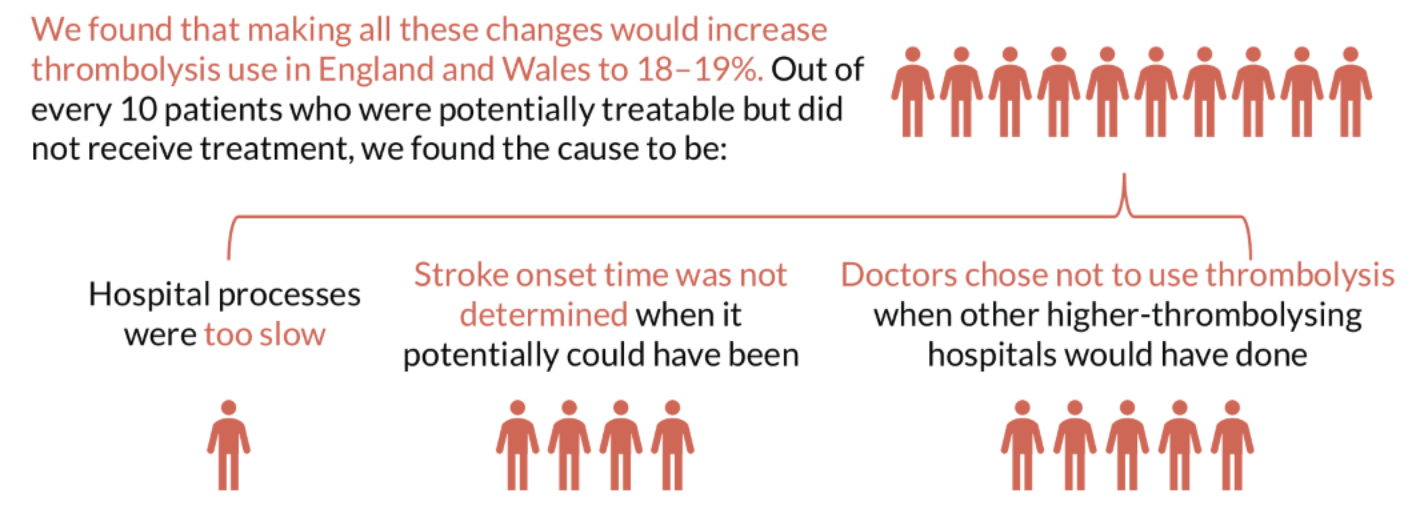
\includegraphics[width=1.0\textwidth]{./images/sam_summary_pt_3}
\end{center}
\end{frame}

%%%%%%%%%%%%%%%%%%%%%%%%%%%%%%%%%%%%%%%%%%%%%%%%%%%%%%%%%%%%%%%

\begin{frame}
\frametitle{Applying our models at hospital level}

\begin{center}
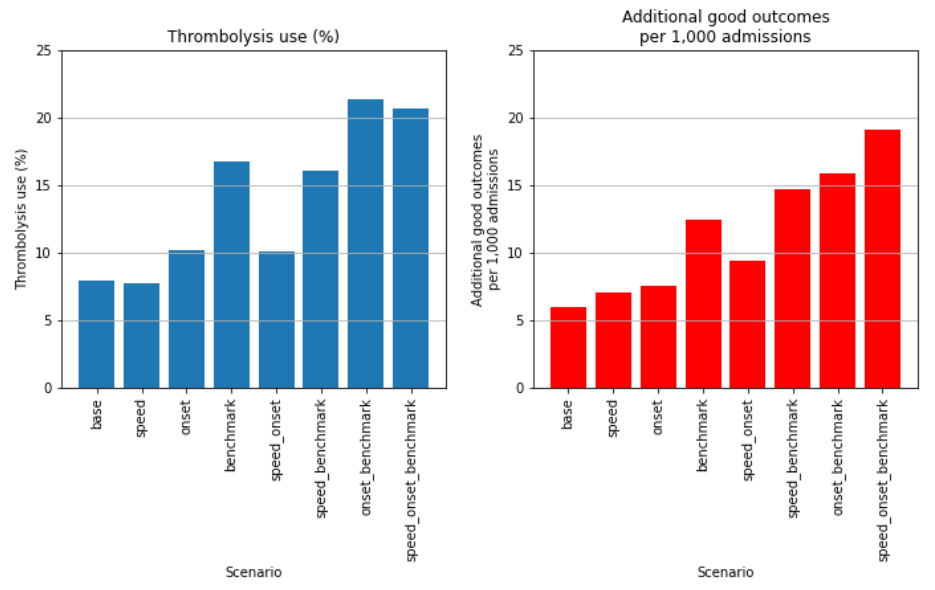
\includegraphics[width=0.95\textwidth]{./images/hosp_scenario_1}
\end{center}

\end{frame}

%%%%%%%%%%%%%%%%%%%%%%%%%%%%%%%%%%%%%%%%%%%%%%%%%%%%%%%%%%%%%%%

\begin{frame}
\frametitle{Machine learning overview}
\begin{center}
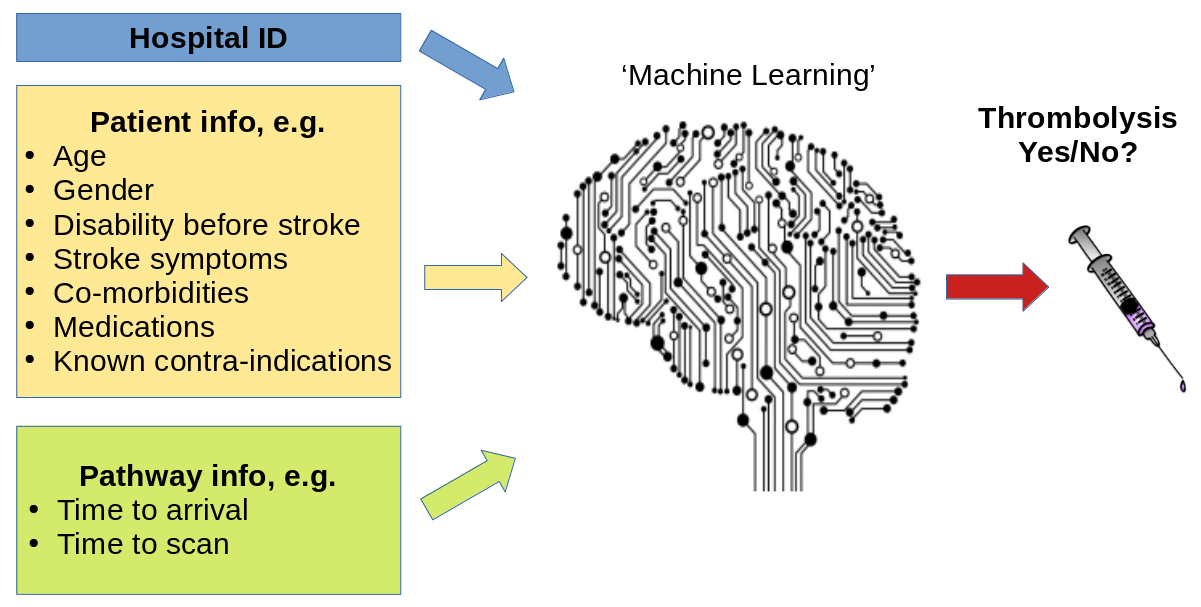
\includegraphics[width=0.90\textwidth]{./images/ml_model_high_level}
\end{center}

\footnotesize
Machine learning (and nearly all \emph{artificial intelligence}) is based on the simple principle of recognising similarity to what has been seen before.
\vspace{3mm}

We accessed 240,000 emergency stroke admissions in England and Wales over three years.
\end{frame}

%%%%%%%%%%%%%%%%%%%%%%%%%%%%%%%%%%%%%%%%%%%%%%%%%%%%%%%%%%%%%%%

\begin{frame}{Model accuracy, and simplification}

Our machine learning models use XGBoost classification, and are based on all patients who arrive within 4 hours of known stroke onset.

\vspace{5mm}

\begin{columns}[T] % [T] Top aligns columns

    \begin{column}{0.5\textwidth}
    
        The full model has 61 patient features:
        
        \begin{footnotesize}
        \begin{itemize}
            \item Overall accuracy = 85.2\%
            \item Best combined sensitivity and specificity = 84.3\%
            \item ROC AUC = 0.921
        \end{itemize}
        \end{footnotesize}
        
        \vspace{3mm}
        
        A simplified model with 8 features
        
        \begin{footnotesize}
        \begin{itemize}
            \item Overall accuracy = 84.8\%
            \item Best combined sensitivity and specificity = 83.8\%
            \item ROC AUC = 0.916
        \end{itemize}
        \end{footnotesize}
    \end{column}
    
    \begin{column}{0.5\textwidth}
    The 8 features of the simplified model are:
        \begin{footnotesize}
        \begin{enumerate}
            \item Arrival-to-scan time
            \item Stroke type (infarction/haemorrhage)
            \item Stroke severity (NIHSS)
            \item Precise or estimated stroke onset time
            \item Prior disability level (mRS)
            \item Stroke team
            \item Use of AF anticoagulants
            \item Onset-to-arrival time
        \end{enumerate}
        \end{footnotesize}
        
    \vspace{2mm}
    \tiny{There are only very weak correlations between the selected features with no R-squared being greater than 0.05.}
    \end{column}
    
\end{columns}
\end{frame}

%%%%%%%%%%%%%%%%%%%%%%%%%%%%%%%%%%%%%%%%%%%%%%%%%%%%%%%%%%%%%%%

\begin{frame}
\frametitle{Explaining model predictions with SHAP values}

SHAP values show the influence of features (even for \emph{`black box'} models).

\begin{center}
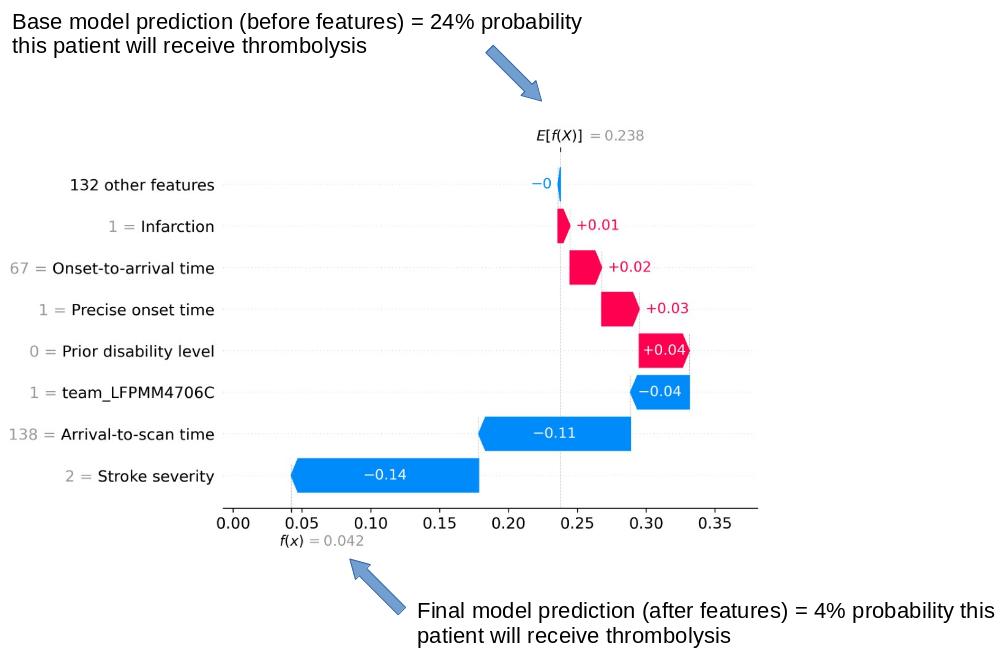
\includegraphics[width=0.85\textwidth]{./images/waterfall_example}
\end{center}
\end{frame}


%%%%%%%%%%%%%%%%%%%%%%%%%%%%%%%%%%%%%%%%%%%%%%%%%%%%%%%%%%%%%%%

\begin{frame}
\frametitle{What drives use of thrombolysis across all hospitals?}

\footnotesize{Note: SHAP values here are \emph{log odds}. Each step-change in value of \textpm 1 changes the chances of receiving thrombolysis about 3-fold. (Plots are in order of feature importance.)}

\begin{center}
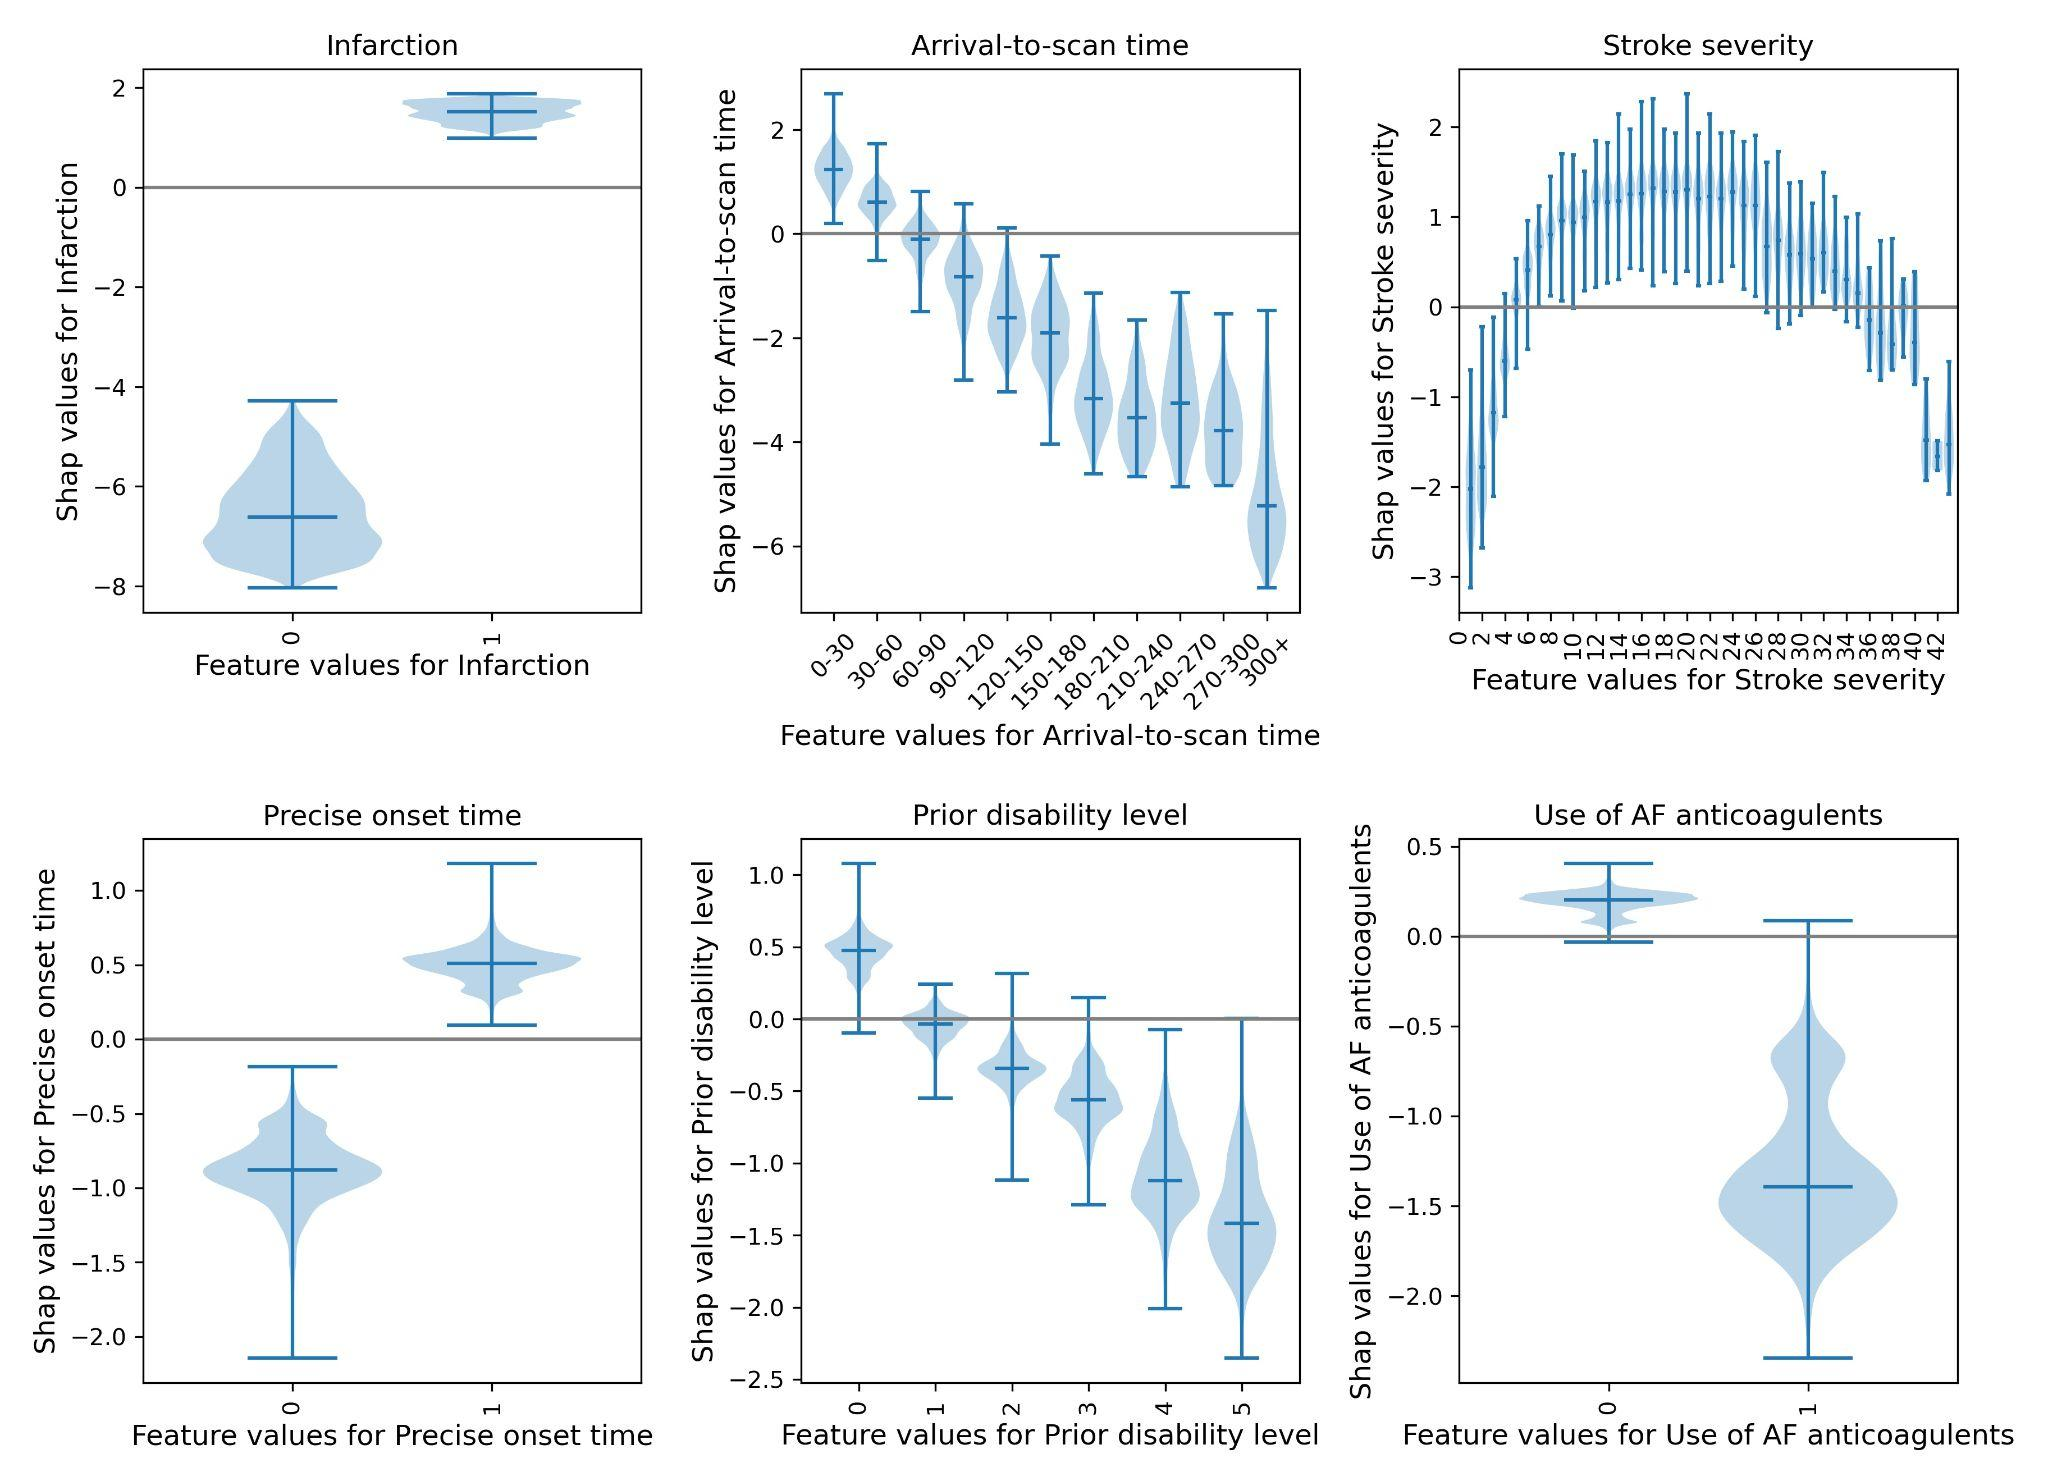
\includegraphics[width=0.80\textwidth]{./images/shap_violins}
\end{center}
\end{frame}

%%%%%%%%%%%%%%%%%%%%%%%%%%%%%%%%%%%%%%%%%%%%%%%%%%%%%%%%%%%%%%%

\begin{frame}
\frametitle{Hospital SHAP values}

\footnotesize
Hospital SHAP values show a hospital's willingness to use thrombolysis.\\
But different patients will have different hospital SHAP values, reflecting the decision-making at each hopsital.

\begin{center}
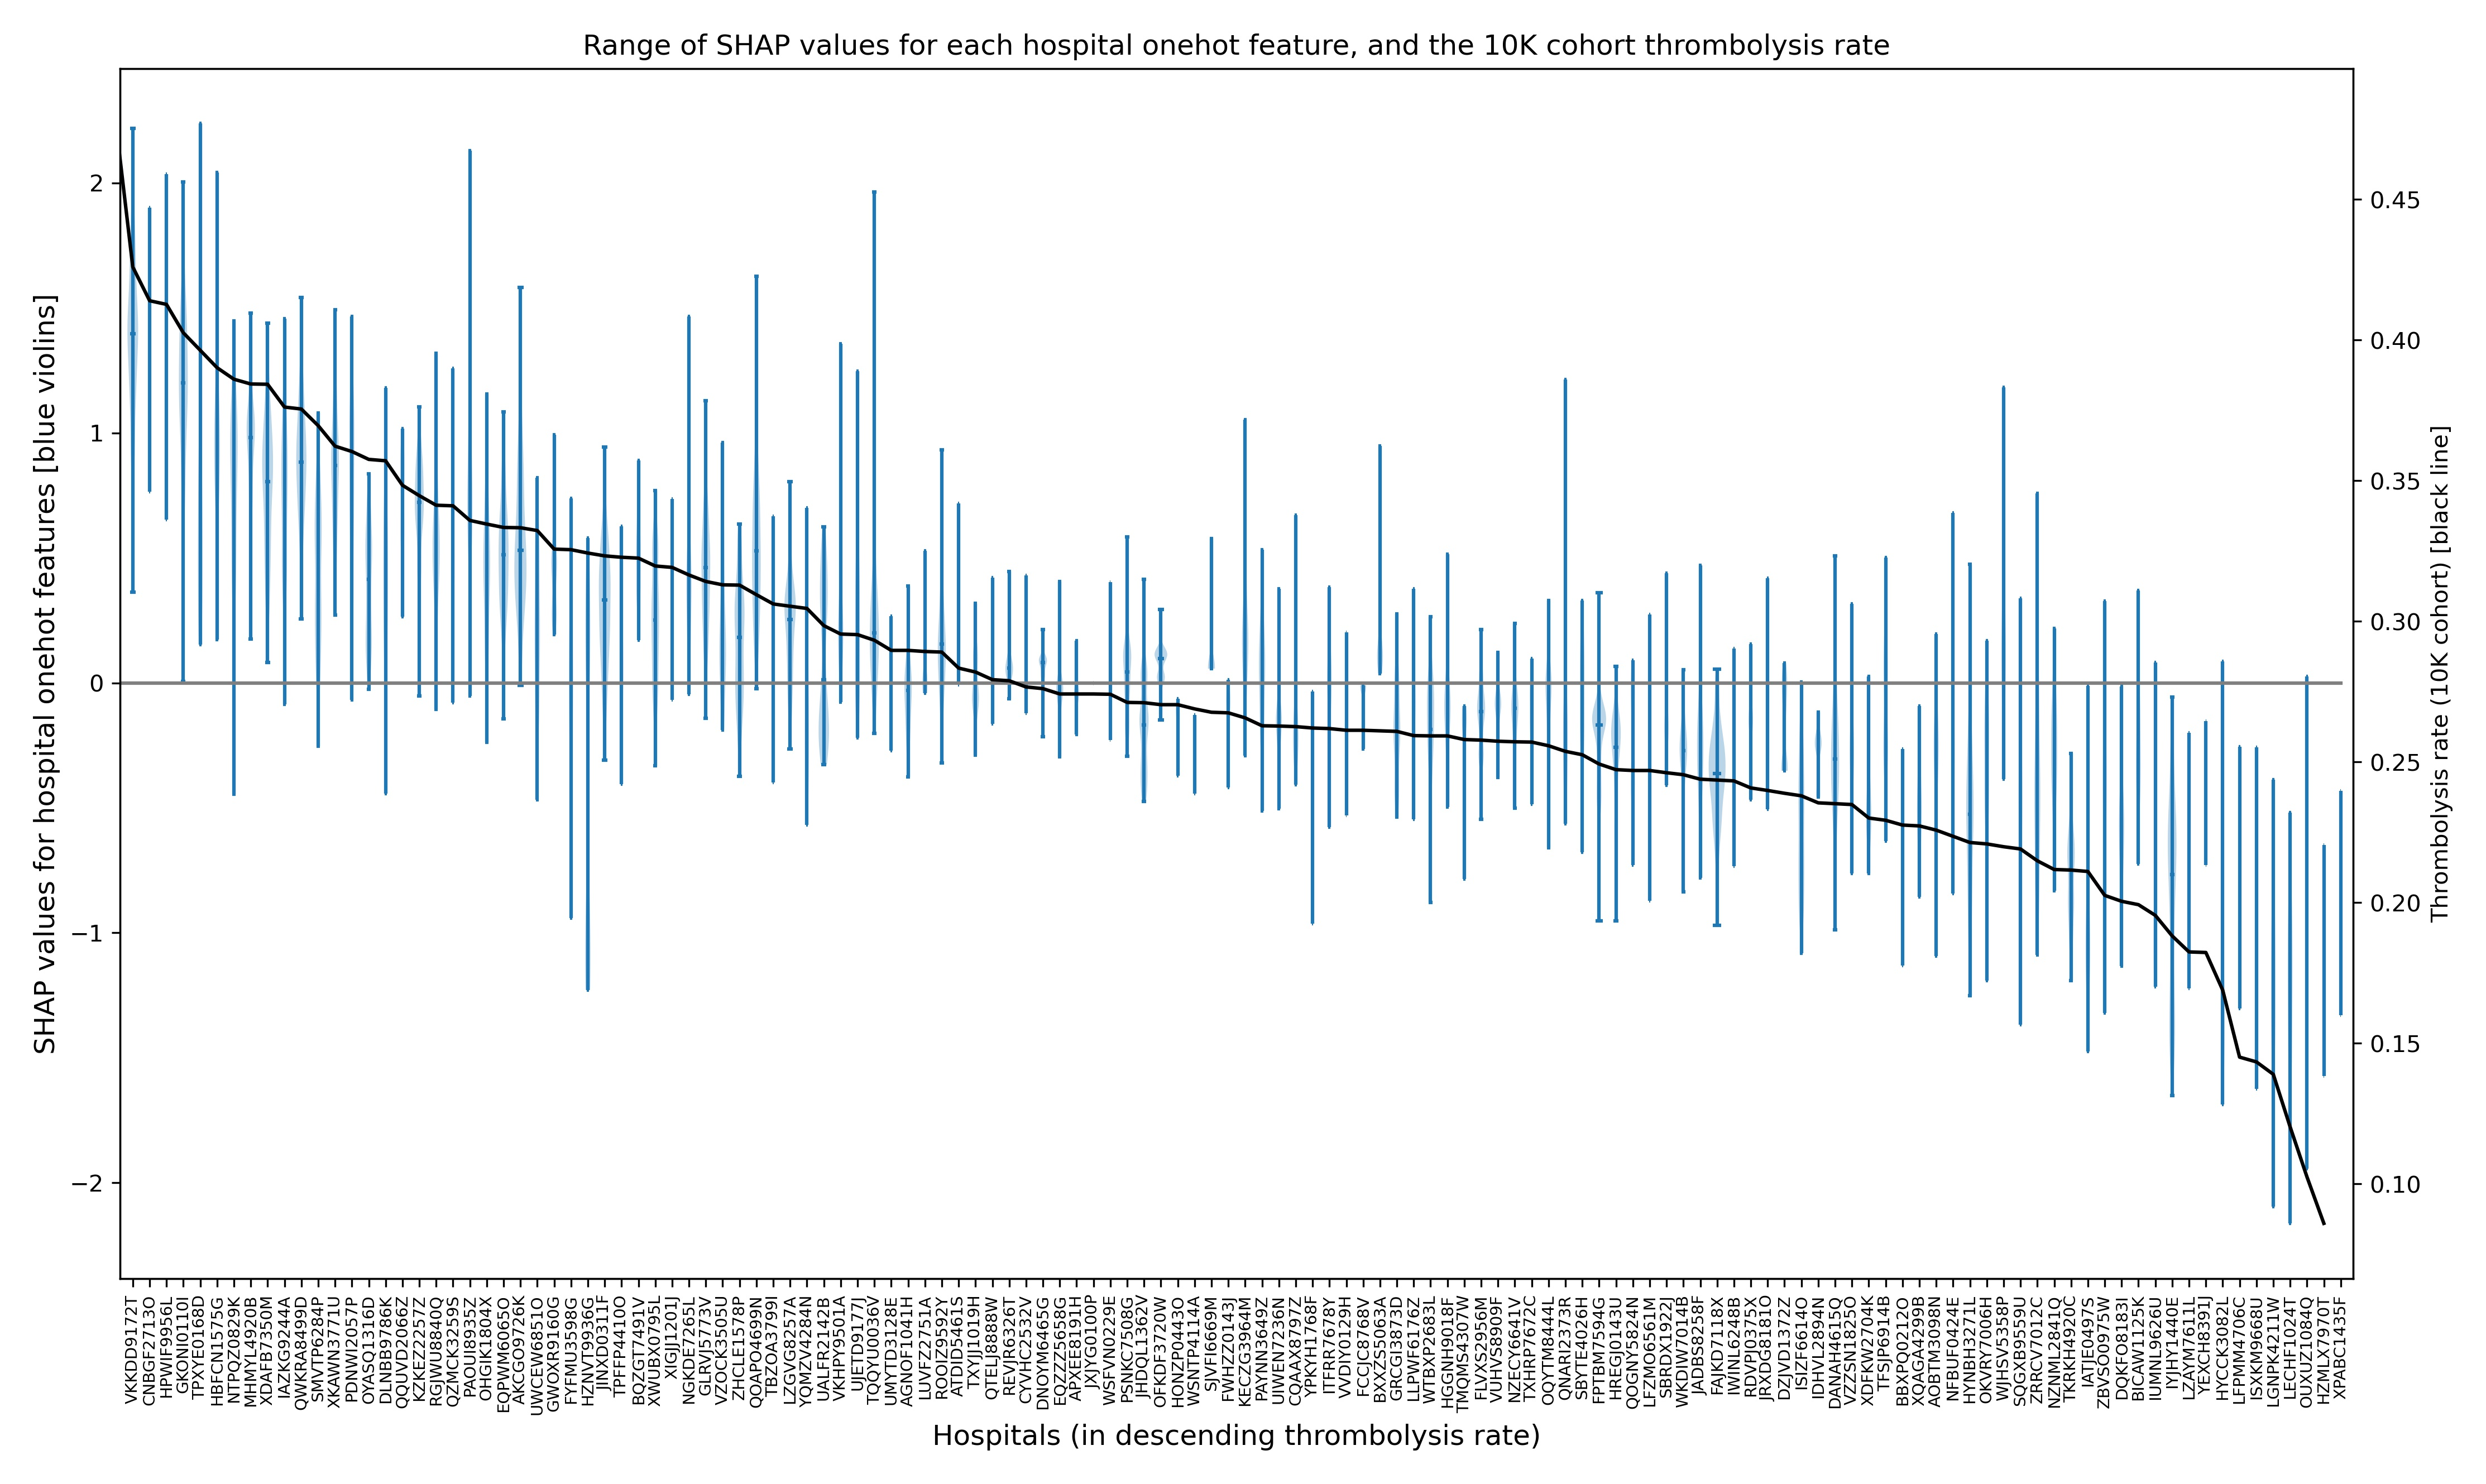
\includegraphics[width=0.90\textwidth]{./images/hospital_feature_shap_violin}
\end{center}
\end{frame}




%%%%%%%%%%%%%%%%%%%%%%%%%%%%%%%%%%%%%%%%%%%%%%%%%%%%%%%%%%%%%%%

\begin{frame}
\frametitle{Investigating how hospitals differ in thrombolysis decision-making: artificial patients}

\vspace{3mm}

\begin{columns}[t]
    \begin{column}{0.45\textwidth}
        Base patient:
        \begin{itemize}
            \footnotesize
            \item Onset to arrival = 80 mins
            \item Arrival to scan = 20 mins
            \item Infarction = Yes
            \item NIHSS = 15
            \item Prior disability level = 0
            \item \emph{Precise onset time = Yes}
            \item Use of AF anticoagulents = No
        \end{itemize}
    \end{column}
    
    \begin{column}{0.5\textwidth}
    Proportion of hospitals predicted to give thrombolysis:
    \footnotesize
    \begin{itemize}
        \item Base patient: 99\%
        \item NIHSS = 4: 73\%
        \item Pre-stroke mRS=3: 86\%
        \item Estimated stroke onset time: 64\%
    \end{itemize}
    \end{column}

\end{columns}
\end{frame}

%%%%%%%%%%%%%%%%%%%%%%%%%%%%%%%%%%%%%%%%%%%%%%%%%%%%%%%%%%%%%%%
\section{Open Science Tooling in Stroke Work}

\begin{frame}{Caveats}

\begin{itemize}
    \setlength\itemsep{1mm}
    \item You may know all of this!
    \item Learning these tools takes time
    \item We are still learning
    \item We still shout at things at times
    \item Other tools exist
    \item These are probably \emph{not} tools for people who's job keeps them in Microsoft Office most of the day
\end{itemize}

\vspace{2mm}
But.....
\vspace{2mm}

\begin{itemize}
    \setlength\itemsep{1mm}
    \item It works; we've used Linux/FOSS for 5+ years
    \item We just use free/open tools
    \item The benefits, and quality of what may be produced, far outweigh the challenges
\end{itemize}

\end{frame}

%%%%%%%%%%%%%%%%%%%%%%%%%%%%%%%%%%%%%%%%%%%%%%%%%%%%%%%%%%%%%%%

\begin{frame}{Our stack of tools}


\begin{center}
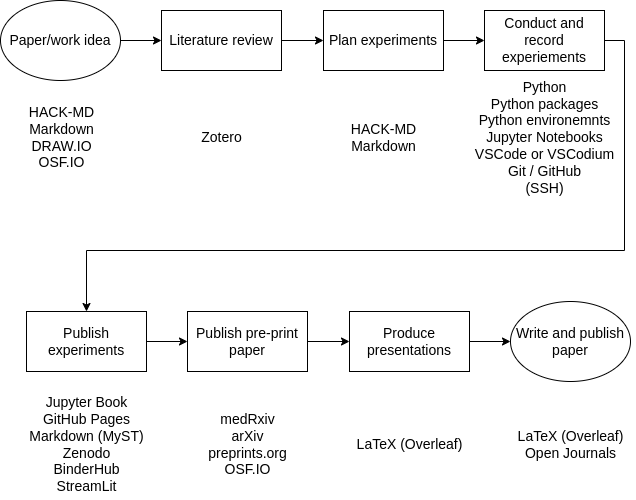
\includegraphics[width=0.75\textwidth]{./images/open_science-2}
\end{center}

\end{frame}

%%%%%%%%%%%%%%%%%%%%%%%%%%%%%%%%%%%%%%%%%%%%%%%%%%%%%%%%%%%%%%%

\begin{frame}{Examples of tools}

\footnotesize

\begin{itemize}
    \item \textcolor{red}{Jupyter Book \& Notebooks:} 
    \smallurl{https://samuel-book.github.io/stroke_outcome/intro.html}
    \item \textcolor{red}{GitHub:} 
    \smallurl{https://github.com/samuel-book/stroke_outcome}
    \item \textcolor{red}{Zenodo:} 
    \smallurl{https://zenodo.org/account/settings/github/}
    \item \textcolor{red}{VS Code}
    \item \textcolor{red}{Overleaf:}
    \smallurl{https://www.overleaf.com/project/630f1aaad6a9ffb27b51490a}
    \item \textcolor{red}{HackMD: }
    \smallurl{https://hackmd.io/@N4jCROVmS9SqGmgj3U66XA/HJPwxmtSs}
    \item \textcolor{red}{Zotero: }
    \smallurl{https://www.zotero.org/groups/4707796/mja_stroke/items/H5JR5N99/library}
    \item \textcolor{red}{Open Print Servers:}
    \smallurl{https://www.medrxiv.org/content/10.1101/2020.07.18.20156653v2}
    \item \textcolor{red}{OSF (Open Science Framework):}
    \smallurl{https://osf.io/dashboard}
    \item \textcolor{red}{Streamlit: }
    \smallurl{https://samuel2-stroke-outcome.streamlit.app/Interactive_demo}
    \item \textcolor{red}{BinderHub: }
    \smallurl{https://github.com/MichaelAllen1966/2004_covid_dialysis}
    
    
\end{itemize}


\end{frame}

%%%%%%%%%%%%%%%%%%%%%%%%%%%%%%%%%%%%%%%%%%%%%%%%%%%%%%%%%%%%%%%

\begin{frame}{General lessons}

\begin{itemize}
    \setlength\itemsep{3mm}
    \item Open Science takes time - quality is not necessarily cheap
        \begin{itemize}
            \item We tend to go through, and refine, notebooks several times to check for errors, make them clear, clean, and understandable
        \end{itemize}
    \item Working with others helps
        \begin{itemize}
            \item We pass notebooks around at times - both for coding and summarising
            \item If a mistake gets through, no single person is to blame
            \item Psychological support
        \end{itemize}
    \item Git can be hard! Allow time to get used to it
    \begin{itemize}
            \item Create a branch for each notebook you work on
            \item Commit and push often
            \item Visual Studio Code has nice Git and GitHub integration (sorry Tom)
        \end{itemize}
    \item If you are new to \LaTeX, don't start with presentations (or posters)
\end{itemize}

\end{frame}

%%%%%%%%%%%%%%%%%%%%%%%%%%%%%%%%%%%%%%%%%%%%%%%%%%%%%%%%%%%%%%%
\section{The PenCHORD Way?}

\begin{frame}{The PenCHORD Way?}

\begin{itemize}
    \setlength\itemsep{3mm}
    \item Do we want a set of tools we more actively support and train people in?
    \item \emph{Supportive} not \emph{coercive}
    \item If so, what tools?
    \item What documentation/training/support material?
    \begin{itemize}
        \item Jupyter Book?
        \item \emph{Mattermost} (FOSS Slack alternative for shared online 'live' support
        \item Other?
    \end{itemize}
    \item What gaps do we have?
    \item How do we involve everyone in developing the PenCHORD Way?
\end{itemize}

\end{frame}

\end{document}


